


\documentclass[12pt,a4paper]{article}

\usepackage[T1]{fontenc}
\usepackage[utf8]{inputenc}
\usepackage{lmodern}
\usepackage{microtype}
\usepackage[a4paper,margin=2.5cm]{geometry}
\usepackage{amsmath,amssymb}
\usepackage{array,booktabs}
\usepackage{xcolor}
\usepackage{setspace}
\usepackage[hidelinks]{hyperref}
\usepackage{tikz}
\usetikzlibrary{arrows.meta,positioning}

\setlength{\parindent}{1.3em}
\setlength{\parskip}{0pt}
\setlength{\emergencystretch}{2em}
\newcolumntype{P}[1]{>{\raggedright\arraybackslash}p{#1}}

\begin{document}
	
	\begin{center}
		{\Large\bfseries Physics-guided placement of conductive particles in a
			polydisperse packed bed\par}
		\vspace{1.0em}
		{\normalsize Ali Khalifa and .....\par}
		\vspace{0.45em}
		{\small Technical University of Munich, Freising, Germany}
	\end{center}
	
	\vspace{1em}
	\setstretch{1.35}
	
	\begin{abstract}
		A granular bed containing a limited amount of conductive material can have
		different thermal performance depending on where that material is placed. We
		study this placement effect without changing the packing geometry, porosity,
		particle-size distribution or conductive-material volume. Ten independent
		500-particle packings were generated by the discrete-element method at a
		nominal porosity of 0.38. A steady contact-network model was then used to
		compare random placement, contact-degree ranking, a heat-path ranking and a
		fixed-budget swap search. Every heterogeneous case contained exactly 10, 30
		and 10 conductive particles from the 1.5, 2.0 and 2.5~mm size classes,
		respectively. Across the ten packings, random placement gave
		$k_{\mathrm{eff}}=0.11046\pm0.00413$~W\,m$^{-1}$\,K$^{-1}$. Degree ranking
		improved this value by only 2.4\% on average, whereas heat-path ranking improved
		it by 10.5\%. The best assignments found by a fixed computational search budget
		improved effective conductivity by $56.3\pm4.1$\% relative to the random mean;
		the improvement was between 50.8\% and 60.9\% in every packing. Independent
		thermal calculations reproduced all reported best values exactly, with maximum
		relative energy-balance error below $3.1\times10^{-12}$. The results show that
		conductive particles are most useful when they cooperate to form effective
		hot-to-cold pathways; selecting locally well-connected particles alone is not
		sufficient. In a representative packing, optimization converted 35 mostly
		small conductive clusters into five clusters, including two wall-spanning
		clusters, and increased the fraction of contact heat carried by
		high--high contacts from 4.6\% to 41.3\%. The present conclusions concern
		stationary, contact-dominated beds and do not yet include a validated
		pore-fluid conduction model.
	\end{abstract}
	
	\noindent\textbf{Keywords:} packed bed; granular heat conduction; discrete
	element method; contact network; material allocation; inverse design
	
	\section{Introduction}
	
	Heat transfer through a packed bed depends on particle conductivity, particle
	size, porosity, contact area and the organization of the contact network.
	Classical theory and thermal discrete-element models describe how these factors
	determine heat flow through a specified granular structure
	\cite{Batchelor1977,Vargas2001,Kiani2019,Joulin2020}. Most such calculations are
	forward problems: the packing and material distribution are prescribed, and
	the resulting temperature field or effective conductivity is calculated.
	
	Many engineering beds, however, contain a limited amount of an expensive or
	specialized conductive phase. In that situation, the practical question is not
	only how much conductive material is present, but where it should be placed.
	Random mixing can put conductive particles in regions that carry little net
	heat. Selecting particles with many contacts may also be inefficient, because a
	highly connected particle can lie on a side branch rather than on a route that
	links the hot and cold boundaries.
	
	Inverse design on graph-structured materials has been considered for
	architected lattices \cite{Dold2023}. A packed bed creates a different problem:
	the graph is not freely drawn or deformed, but is the mechanically admissible
	contact network produced by particle packing. The geometry remains fixed and
	only the particle material labels are changed. This gives a controlled question:
	
	\begin{quote}
		At fixed porosity, particle-size distribution and conductive-material volume,
		can the effective conductivity of a packed bed be increased substantially by
		placing conductive particles according to the global heat-transfer network?
	\end{quote}
	
	We address this question using ten independent DEM packings, a verified steady
	thermal contact network and four increasingly informed allocation strategies.
	The study deliberately begins without machine learning. A learned graph policy
	is useful only if the physical allocation effect is reproducible and if a
	transparent method does not already solve the problem sufficiently well.
	
	Figure~\ref{fig:problem} summarizes the physical problem. DEM first fixes the
	particle positions and contacts. The material budget is then allocated without
	moving any particle or changing the packing porosity and particle-size
	distribution. The present paper considers heat conduction through solid
	contacts only; stagnant-fluid conduction is reserved for a later, separately
	validated extension.
	
\begin{figure}[!htbp]
	\centering
	\resizebox{0.85\textwidth}{!}{%
		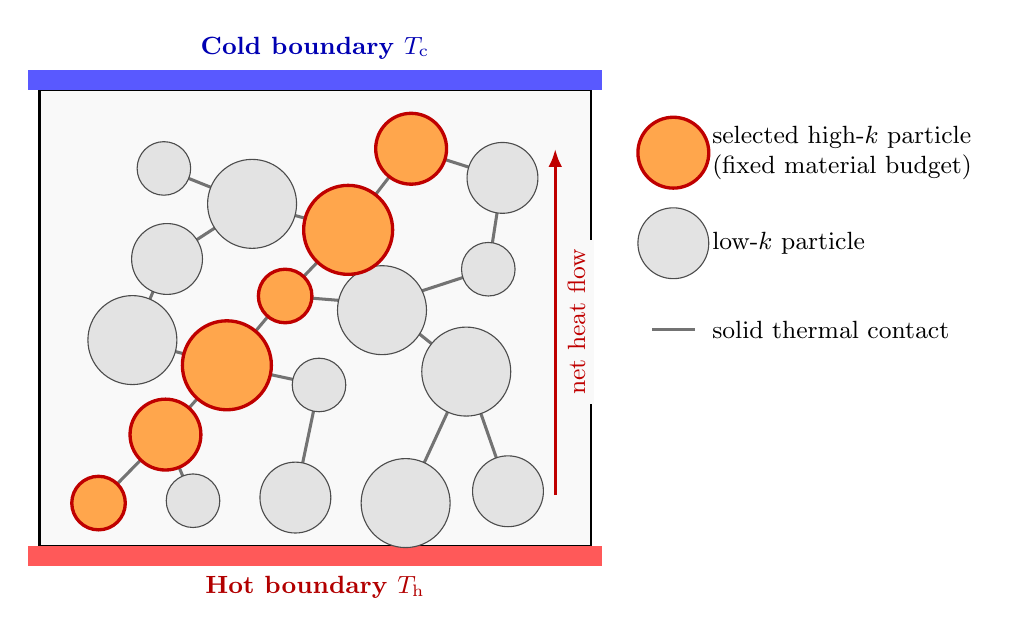
\begin{tikzpicture}[
			% Low-conductivity particles
			particleSmall/.style={
				circle,
				draw=black!70,
				fill=gray!22,
				minimum size=6.8mm,
				inner sep=0pt
			},
			particleMedium/.style={
				circle,
				draw=black!70,
				fill=gray!22,
				minimum size=9.0mm,
				inner sep=0pt
			},
			particleLarge/.style={
				circle,
				draw=black!70,
				fill=gray!22,
				minimum size=11.3mm,
				inner sep=0pt
			},
			% High-conductivity particles
			conductiveSmall/.style={
				circle,
				draw=red!75!black,
				very thick,
				fill=orange!70,
				minimum size=6.8mm,
				inner sep=0pt
			},
			conductiveMedium/.style={
				circle,
				draw=red!75!black,
				very thick,
				fill=orange!70,
				minimum size=9.0mm,
				inner sep=0pt
			},
			conductiveLarge/.style={
				circle,
				draw=red!75!black,
				very thick,
				fill=orange!70,
				minimum size=11.3mm,
				inner sep=0pt
			},
			contact/.style={
				draw=black!55,
				line width=1.1pt
			},
			heat/.style={
				-{Latex[length=2.3mm]},
				red!75!black,
				very thick
			},
			labelbox/.style={
				align=left,
				font=\small
			}
			]
			
			% Packed-bed domain and thermal boundaries
			\fill[gray!5] (0,0) rectangle (7,5.8);
			\draw[thick] (0,0) rectangle (7,5.8);
			
			\fill[red!65] (-0.15,-0.25) rectangle (7.15,0);
			\fill[blue!65] (-0.15,5.8) rectangle (7.15,6.05);
			
			\node[
			font=\small\bfseries,
			red!70!black
			] at (3.5,-0.52)
			{Hot boundary $T_{\mathrm h}$};
			
			\node[
			font=\small\bfseries,
			blue!70!black
			] at (3.5,6.33)
			{Cold boundary $T_{\mathrm c}$};
			
			% Particle-contact network
			\draw[contact]
			(0.75,0.55)--(1.60,1.42)--(2.38,2.30)--
			(3.12,3.18)--(3.92,4.02)--(4.72,5.05);
			
			\draw[contact] (1.95,0.58)--(1.60,1.42);
			\draw[contact] (2.38,2.30)--(1.18,2.62);
			\draw[contact] (2.38,2.30)--(3.55,2.05);
			\draw[contact] (3.12,3.18)--(4.35,3.08);
			\draw[contact] (3.92,4.02)--(2.70,4.35);
			\draw[contact] (4.72,5.05)--(5.88,4.68);
			
			% Additional low-conductivity contacts
			\draw[contact] (3.25,0.62)--(3.55,2.05);
			\draw[contact] (4.65,0.55)--(5.42,2.22);
			\draw[contact] (5.95,0.70)--(5.42,2.22);
			\draw[contact] (1.18,2.62)--(1.62,3.65);
			\draw[contact] (1.62,3.65)--(2.70,4.35);
			\draw[contact] (4.35,3.08)--(5.42,2.22);
			\draw[contact] (4.35,3.08)--(5.70,3.52);
			\draw[contact] (5.70,3.52)--(5.88,4.68);
			\draw[contact] (2.70,4.35)--(1.58,4.80);
			
			% Low-conductivity particles: three size classes
			\node[particleSmall]  at (1.95,0.58) {};
			\node[particleMedium] at (3.25,0.62) {};
			\node[particleLarge]  at (4.65,0.55) {};
			\node[particleMedium] at (5.95,0.70) {};
			
			\node[particleLarge]  at (1.18,2.62) {};
			\node[particleSmall]  at (3.55,2.05) {};
			\node[particleLarge]  at (5.42,2.22) {};
			
			\node[particleMedium] at (1.62,3.65) {};
			\node[particleLarge]  at (4.35,3.0) {};
			\node[particleSmall]  at (5.70,3.52) {};
			
			\node[particleLarge]  at (2.70,4.35) {};
			\node[particleSmall]  at (1.58,4.80) {};
			\node[particleMedium] at (5.88,4.68) {};
			
			% Selected high-conductivity particles
			\node[conductiveSmall]  at (0.75,0.55) {};
			\node[conductiveMedium] at (1.60,1.42) {};
			\node[conductiveLarge]  at (2.38,2.30) {};
			\node[conductiveSmall]  at (3.12,3.18) {};
			\node[conductiveLarge]  at (3.92,4.02) {};
			\node[conductiveMedium] at (4.72,5.05) {};
			
			% Net heat-flow direction
			\draw[heat] (6.55,0.65)--(6.55,5.05);
			
			\node[
			font=\small,
			rotate=90,
			red!75!black,
			fill=gray!5
			] at (6.82,2.85)
			{net heat flow};
			
			% Material legend
			\node[conductiveMedium] at (8.05,5.00) {};
			
			\node[
			labelbox,
			anchor=west
			] at (8.42,5.00)
			{selected high-$k$ particle\\
				(fixed material budget)};
			
			\node[particleMedium] at (8.05,3.85) {};
			
			\node[
			labelbox,
			anchor=west
			] at (8.42,3.85)
			{low-$k$ particle};
			
			% Contact legend
			\draw[contact] (7.78,2.75)--(8.32,2.75);
			
			\node[
			labelbox,
			anchor=west
			] at (8.42,2.75)
			{solid thermal contact};
			
			% Particle-size legend
%			\node[
%			labelbox,
%			anchor=west,
%			font=\small\bfseries
%			] at (7.75,1.80)
%			{Particle-size classes:};
%			
%			\node[particleSmall] at (8.02,1.20) {};
%			\node[particleMedium] at (9.20,1.20) {};
%			\node[particleLarge] at (10.55,1.20) {};
%			
%			\node[
%			font=\scriptsize,
%			anchor=north
%			] at (8.02,0.85)
%			{$1.5$ mm};
%			
%			\node[
%			font=\scriptsize,
%			anchor=north
%			] at (9.20,0.75)
%			{$2.0$ mm};
%			
%			\node[
%			font=\scriptsize,
%			anchor=north
%			] at (10.55,0.65)
%			{$2.5$ mm};
%			
			% Fixed-geometry explanation
%			\node[
%			labelbox,
%			anchor=west,
%			text width=4.2cm
%			] at (7.78,-0.10)
%			{DEM fixes particle positions, particle sizes and contact topology.
%				Only the material labels are changed.};
%			
		\end{tikzpicture}%
	}
	
	\caption{Schematic of the inverse allocation problem for a polydisperse packed
		bed. The three illustrated particle sizes represent the simulated diameter
		classes of 1.5, 2.0 and 2.5~mm. DEM fixes the particle positions, particle-size
		distribution and contact network. A prescribed number of particles from each
		size class receives the high-conductivity material, while the packing geometry
		and total conductive-material volume remain unchanged. Heat is conducted
		through the fixed solid-contact network.}
	
	\label{fig:problem}
\end{figure}
	
	\section{Methods}
	
	\subsection{Controlled DEM packing ensemble}
	
	The packings were generated with LAMMPS using a Hertz--Mindlin granular contact
	model \cite{LAMMPSGranular}. Each realization contains 500 spherical particles
	in a cubic domain with periodic boundaries in the horizontal directions and
	fixed walls in the vertical direction. The number-based particle-size
	distribution is identical in every realization: 100 particles of diameter
	1.5~mm, 300 of diameter 2.0~mm and 100 of diameter 2.5~mm. The cubic cell size
	was calculated from the exact undeformed particle volume to impose a nominal
	porosity of 0.38.
	
	Ten random seeds generated ten different center arrangements and contact
	networks. All particle counts, sizes, material properties, cell dimensions,
	growth settings and relaxation settings were held fixed. The resulting contact
	graphs contained 1325--1382 particle--particle contacts. Every packing had one
	component that connected the lower and upper walls.
	
	\subsection{Steady thermal contact network}
	
	Each particle is represented by a graph node and every DEM contact by a thermal
	edge. For an internal particle $i$, steady energy conservation is
	\begin{equation}
		\sum_{j\in\mathcal N_i}G_{ij}(T_j-T_i)=0,
		\label{eq:balance}
	\end{equation}
	where $G_{ij}$ is the contact conductance. For two particles with conductivities
	$k_i$ and $k_j$ and contact radius $a_{ij}$, the constriction model is
	\begin{equation}
		G_{ij}=\frac{2a_{ij}k_i k_j}{k_i+k_j},
		\qquad
		a_{ij}=\sqrt{R_{ij}^{*}\delta_{ij}},
		\label{eq:conductance}
	\end{equation}
	where $R_{ij}^{*}=R_iR_j/(R_i+R_j)$ and $\delta_{ij}$ is the DEM overlap. Fixed
	temperatures of 301 and 300~K were applied at the lower and upper walls. The
	effective conductivity follows from
	\begin{equation}
		k_{\mathrm{eff}}=\frac{QH}{A(T_{\mathrm h}-T_{\mathrm c})},
		\label{eq:keff}
	\end{equation}
	where $Q$ is the wall heat rate, $H$ is bed height and $A$ is cross-sectional
	area.
	
	The present paper uses solid-contact conduction only. A preliminary stagnant-air
	gap model was tested, but its predicted conductivity depended too strongly on
	an arbitrary neighbour cutoff. Those results were therefore excluded from the
	allocation conclusions. This choice makes the present scope a stationary,
	contact-dominated bed rather than a flowing or convective system.
	
	\subsection{Fixed material budget}
	
	The low- and high-conductivity materials were assigned
	$k_{\mathrm L}=1$ and $k_{\mathrm H}=10$~W\,m$^{-1}$\,K$^{-1}$. A binary
	variable $x_i$ indicates whether particle $i$ receives the high-conductivity
	material:
	\begin{equation}
		k_i=k_{\mathrm L}+x_i(k_{\mathrm H}-k_{\mathrm L}).
	\end{equation}
	
	Because the bed is polydisperse, selecting the same total number of particles
	does not automatically select the same material volume. Every allocation was
	therefore constrained to contain 10 small, 30 medium and 10 large
	high-conductivity particles. The selected conductive-particle volume was
	$2.2514747\times10^{-7}$~m$^3$ in every calculation. This constraint preserves
	both the conductive-particle count and its size distribution.
	
	\subsection{Allocation strategies}
	
	Four strategies were compared on every fixed packing:
	
	\begin{enumerate}
		\item \textbf{Random placement:} 100 independent assignments satisfying the
		size-class quotas. Their mean and standard deviation define the undesigned
		reference.
		\item \textbf{Degree ranking:} within each size class, particles with the most
		contacts are selected first.
		\item \textbf{Heat-path ranking:} the homogeneous low-conductivity bed is
		solved first. Each particle receives the score
		\begin{equation}
			S_i=\sum_j\left|G_{ij}(T_i-T_j)\right|,
		\end{equation}
		which measures the baseline heat passing through its incident contacts. The
		highest-scoring particles are selected within each size class.
		\item \textbf{Fixed-budget single-swap search:} the search starts from the
		better of degree and heat-path ranking. One selected and one unselected
		particle of the same size class are exchanged. The exchange is retained only
		when it increases $k_{\mathrm{eff}}$. Five independent restarts with 3000
		proposed swaps each were used.
	\end{enumerate}
	The swap search is a simple local-search method based on exchanging two
	particles. In each proposal, one high-conductivity particle and one
	low-conductivity particle from the same size class exchange their material
	labels. This preserves the number, size distribution and total volume of the
	high-conductivity particles. The new allocation is accepted only if it
	increases $k_{\mathrm{eff}}$. Similar exchange strategies are widely used in
	combinatorial optimization
	\cite{KernighanLin1970,Maringer2003}, although our implementation is adapted
	specifically to the packed-bed thermal problem. Because only a fixed number of
	exchanges is tested, the method identifies a good allocation but does not
	guarantee the global optimum. Performance is evaluated relative to the mean
	result obtained from random allocations in the same packing:
	\begin{equation}
		I=100\frac{k_{\mathrm{eff}}-\overline{k}_{\mathrm{eff,random}}}
		{\overline{k}_{\mathrm{eff,random}}}\;[\%].
		\label{eq:improvement}
	\end{equation}
	
	\subsection{Numerical verification and statistical reporting}
	
	The sparse solver was tested for energy conservation and linear scaling. On a
	representative packing, doubling all particle conductivities doubled both heat
	rate and $k_{\mathrm{eff}}$. Increasing the imposed temperature difference by
	a factor of ten increased heat rate by ten while leaving $k_{\mathrm{eff}}$
	unchanged. Temperatures remained between the boundary values.
	
	The ten DEM realizations are treated as independent packing samples. Results
	are reported as mean $\pm$ sample standard deviation. For the improvement over
	random placement, a 95\% confidence interval was calculated with the Student
	$t$ distribution. Each best particle-ID assignment was also passed to an
	independent call of the thermal solver.
	
	The complete computational workflow is shown in Fig.~\ref{fig:workflow}. DEM is
	required only once for each packing. The same contact graph can subsequently be
	evaluated for many material allocations, which makes controlled comparison and
	fixed-budget search possible without regenerating the packing.
	
	\begin{figure}[!htbp]
		\centering
		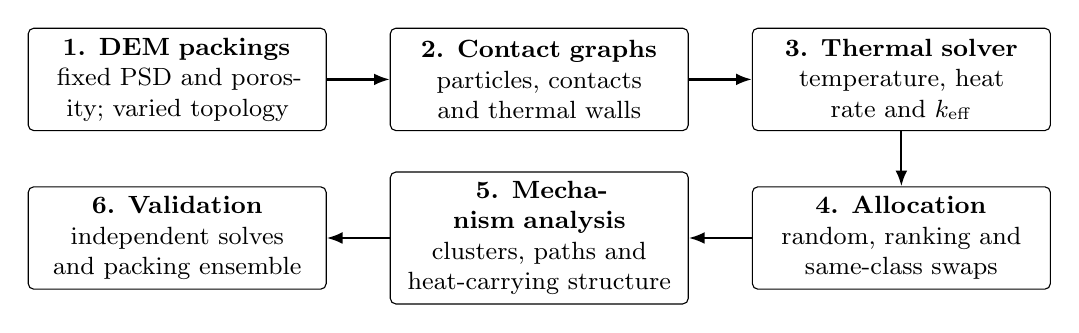
\begin{tikzpicture}[
			node distance=7mm and 8mm,
			box/.style={draw,rounded corners=2pt,align=center,minimum height=13mm,text width=3.55cm,font=\small},
			arrow/.style={-{Latex[length=2mm]},thick}
			]
			\node[box] (dem) {\textbf{1. DEM packings}\\fixed PSD and porosity; varied topology};
			\node[box, right=of dem] (graph) {\textbf{2. Contact graphs}\\particles, contacts and thermal walls};
			\node[box, right=of graph] (solver) {\textbf{3. Thermal solver}\\temperature, heat rate and $k_{\mathrm{eff}}$};
			\node[box, below=of solver] (alloc) {\textbf{4. Allocation}\\random, ranking and same-class swaps};
			\node[box, left=of alloc] (mechanism) {\textbf{5. Mechanism analysis}\\clusters, paths and heat-carrying structure};
			\node[box, left=of mechanism] (validation) {\textbf{6. Validation}\\independent solves and packing ensemble};
			\draw[arrow] (dem)--(graph);
			\draw[arrow] (graph)--(solver);
			\draw[arrow] (solver)--(alloc);
			\draw[arrow] (alloc)--(mechanism);
			\draw[arrow] (mechanism)--(validation);
		\end{tikzpicture}
		\caption{Computational workflow. DEM is run once per packing, whereas the
			thermal network is repeatedly solved on the same contact graph to compare
			controlled material allocations and explain their performance.}
		\label{fig:workflow}
	\end{figure}
	
	\section{Results}
	
	\subsection{Homogeneous packing variability}
	
	With all particles assigned $k=1$~W\,m$^{-1}$\,K$^{-1}$, the ten packings gave
	\begin{equation}
		k_{\mathrm{eff,hom}}=0.09329\pm0.00351~\mathrm{W\,m^{-1}K^{-1}}.
	\end{equation}
	The range was 0.08615--0.09717~W\,m$^{-1}$\,K$^{-1}$ and the coefficient of
	variation was 3.77\%. The mean coordination number was
	$5.393\pm0.066$, with a smaller coefficient of variation of 1.22\%. Thus,
	packings with nearly identical contact counts still showed measurable thermal
	variation, indicating that contact arrangement and conductance weights matter.
	
	Between one and eleven particles per packing were outside the wall-anchored
	contact component. They carry no heat in the contact-only model and were
	excluded from the linear system. Every packing nevertheless contained one
	large component spanning both thermal walls.
	
	\subsection{Allocation performance across ten packings}
	
	Table~\ref{tab:summary} shows the ensemble results. Adding 10\% conductive
	particles at random raised the mean conductivity to
	$0.11046\pm0.00413$~W\,m$^{-1}$\,K$^{-1}$. Degree ranking produced only a small
	additional improvement and was slightly worse than the random mean in one
	packing. Heat-path ranking was better than random in all ten packings.
	
	\begin{table}[!htbp]
		\centering
		\caption{Performance across ten independent DEM packings. Improvement is
			calculated relative to the controlled random mean in the same packing.}
		\label{tab:summary}
		\small
		\begin{tabular}{P{4.1cm}P{3.7cm}P{3.7cm}}
			\toprule
			\textbf{Allocation} &
			$\boldsymbol{k_{\mathrm{eff}}}$ \textbf{[W/(m K)]} &
			\textbf{Mean improvement} \\
			\midrule
			Random mean & $0.11046\pm0.00413$ & reference \\
			Degree ranking & $0.11310\pm0.00425$ & $2.4\pm2.5$\% \\
			Heat-path ranking & $0.12208\pm0.00467$ & $10.5\pm2.3$\% \\
			Swap search, five-restart mean & $0.16868\pm0.00692$ & $52.7\pm3.5$\% \\
			Best fixed-budget search & $0.17263\pm0.00787$ & $56.3\pm4.1$\% \\
			\bottomrule
		\end{tabular}
	\end{table}
	
	The best fixed-budget search improved on random placement in every realization.
	The smallest improvement was 50.8\% and the largest was 60.9\%. The mean
	improvement was 56.3\%, with a 95\% confidence interval of 53.4--59.2\%.
	The corresponding improvement over the homogeneous low-conductivity bed was
	$85.1\pm4.9$\%.
	
	\begin{table}[!htbp]
		\centering
		\caption{Per-packing controlled allocation results.}
		\label{tab:cases}
		\small
		\begin{tabular}{rrrrr}
			\toprule
			\textbf{Seed} & \textbf{Random mean} & \textbf{Heat path} &
			\textbf{Best search} & \textbf{Gain [\%]} \\
			\midrule
			18427 & 0.11123 & 0.12186 & 0.17895 & 60.9 \\
			29173 & 0.10194 & 0.11045 & 0.15600 & 53.0 \\
			37811 & 0.11317 & 0.12510 & 0.18102 & 60.0 \\
			46549 & 0.11216 & 0.12153 & 0.16918 & 50.8 \\
			55291 & 0.11330 & 0.12602 & 0.18219 & 60.8 \\
			64109 & 0.10562 & 0.12018 & 0.16895 & 60.0 \\
			72869 & 0.11075 & 0.12669 & 0.17540 & 58.4 \\
			81647 & 0.11472 & 0.12467 & 0.17498 & 52.5 \\
			90439 & 0.11402 & 0.12369 & 0.17334 & 52.0 \\
			99223 & 0.10774 & 0.12058 & 0.16628 & 54.3 \\
			\bottomrule
		\end{tabular}
	\end{table}
	
	The mean of the five final swap-search values was also substantially above
	random in every packing, with improvements between 48.7\% and 58.1\%. This
	shows that the conclusion does not depend only on selecting the best of five
	search trajectories.
	
	\subsection{Independent reproduction and conservation}
	
	The best ID list from every packing was independently evaluated by the thermal
	solver. All ten values reproduced the allocation-driver results exactly. Every
	independent calculation contained exactly 50 high-conductivity particles and
	the original DEM contact graph. The maximum relative difference between hot-
	and cold-side heat rates was $3.04\times10^{-12}$. These checks rule out output
	rounding, a changed graph or a mismatch in particle IDs as explanations for the
	observed improvement.
	
	\subsection{Mechanism comparison in a representative packing}
	
	To examine why the optimized assignment performs better, seed 18427 was
	analysed in greater detail. Three allocations were compared on exactly the same
	contact graph: a random realization closest to the random mean, heat-path
	ranking and the best fixed-budget swap-search result. The diagnostic quantities
	in Table~\ref{tab:mechanism} describe connections between high-conductivity
	particles, their contact with the thermal walls, and the heat carried by the
	resulting network.
	
	The indicators describe different, complementary aspects of the conductive
	structure. Their definitions and physical meanings are as follows.
	
	\begin{itemize}
		\item \textbf{Effective conductivity, $k_{\mathrm{eff}}$,} is the overall
		thermal performance of the complete packed bed. It is calculated from the
		total heat rate between the hot and cold walls, the imposed temperature
		difference and the bed dimensions. Unlike the remaining indicators, it
		includes the combined effect of all contacts and all parallel heat-transfer
		routes.
		
		\item \textbf{High--high contacts} counts direct particle contacts for which
		both particles have the high conductivity. A larger number means that the
		conductive material is less isolated and has more opportunities to form
		continuous low-resistance routes. The count alone is not sufficient, however,
		because contacts on horizontal side branches may contribute little to heat
		transfer between the two walls.
		
		\item \textbf{High-$k$ clusters} are connected components formed using only
		high-conductivity particles and high--high contacts. Two conductive particles
		belong to the same cluster when they are connected directly or through a chain
		of other conductive particles. Many clusters therefore indicate a fragmented
		conductive phase, whereas fewer clusters indicate that the same 50 particles
		have been consolidated into larger connected structures.
		
		\item \textbf{Largest high-$k$ cluster} is the number of particles in the
		largest of these connected components. It shows whether a substantial part of
		the available conductive material participates in one cooperative structure.
		A large cluster is useful only if it is located and oriented so that it helps
		connect the thermal boundaries.
		
		\item \textbf{Wall-spanning high-$k$ clusters} counts conductive clusters
		that contain at least one particle touching the hot wall and at least one
		particle touching the cold wall. Such a cluster provides an uninterrupted
		sequence of high-conductivity particles across the bed. A value larger than
		one indicates multiple parallel conductive routes rather than a single chain.
		
		\item \textbf{High-$k$ particles linked to the hot/cold wall} gives the number
		of conductive particles in direct thermal contact with each boundary. These
		particles act as entry and exit points for heat. The notation $7/6$, for
		example, means that seven high-$k$ particles touch the hot wall and six touch
		the cold wall. High values at only one wall do not by themselves guarantee a
		complete hot-to-cold route.
		
		\item \textbf{Heat on high--high contacts} is the sum of the absolute heat
		rates through all high--high contacts divided by the corresponding sum over
		all particle--particle contacts. Absolute values are used so that heat rates
		in different edge directions do not cancel. This fraction measures how much
		of the active contact-network heat transport actually uses connections between
		conductive particles. It is therefore more informative than merely counting
		high--high contacts.
		
		\item \textbf{Heat-weighted vertical alignment} describes whether the
		high--high contacts that carry heat are oriented in the direction between the
		hot and cold walls. For each high--high contact, the alignment is
		$|\Delta z|/d_{ij}$, which is zero for a horizontal contact and one for a
		perfectly vertical contact. The reported mean is weighted by the absolute
		heat rate of each contact. A value closer to one therefore means that the most
		active conductive contacts are preferentially aligned with the imposed
		temperature gradient.
		
		\item \textbf{Minimum-path resistance} is obtained by assigning every thermal
		link the resistance $1/G_{ij}$ and finding the hot-to-cold path with the
		smallest sum of link resistances. A smaller value identifies a more favourable
		single route through the contact graph. It is a diagnostic path measure, not
		the total bed resistance, because the full thermal solution also includes many
		parallel and interconnected routes.
		
		\item \textbf{High-$k$ fraction on the minimum path} is the percentage of
		particles on that lowest-resistance path that have high conductivity. A value
		of 100\% means that every particle along the identified particle sequence is
		conductive. This indicator shows whether the material allocation reinforces
		the most favourable individual route, while $k_{\mathrm{eff}}$ remains the
		measure of the performance of the entire network.
	\end{itemize}
	
	The indicators should consequently be interpreted together. Contact and
	cluster counts describe how the conductive phase is connected; wall contact
	and vertical alignment describe whether this connection is useful for the
	imposed heat-flow direction; and the heat fractions and path resistance show
	whether the resulting structure is actually used by the thermal solution.
	
	\begin{table}[!htbp]
		\centering
		\caption{Mechanism comparison for packing seed 18427. The minimum-path
			resistance is a descriptive series-path indicator and not the total resistance
			of the parallel contact network.}
		\label{tab:mechanism}
		\small
		\begin{tabular}{P{5.1cm}rrr}
			\toprule
			\textbf{Indicator} & \textbf{Random} & \textbf{Heat path} & \textbf{Optimized} \\
			\midrule
			$k_{\mathrm{eff}}$ [W/(m K)] & 0.1112 & 0.1219 & \textbf{0.1789} \\
			High--high contacts & 17 & 27 & \textbf{55} \\
			Number of high-$k$ clusters & 35 & 26 & \textbf{5} \\
			Largest high-$k$ cluster [particles] & 6 & 5 & \textbf{26} \\
			Wall-spanning high-$k$ clusters & 0 & 0 & \textbf{2} \\
			High-$k$ particles linked to hot/cold wall & 4/2 & 0/0 & \textbf{7/6} \\
			Heat on high--high contacts [\%] & 4.6 & 9.1 & \textbf{41.3} \\
			Heat-weighted vertical alignment & 0.666 & 0.728 & \textbf{0.804} \\
			Minimum-path resistance [K/W] & 19894 & 15884 & \textbf{2892} \\
			High-$k$ fraction on minimum path [\%] & 63.6 & 55.6 & \textbf{100} \\
			\bottomrule
		\end{tabular}
	\end{table}
	
	The random allocation divided the 50 conductive particles into 35 mostly small
	clusters, and no all-conductive cluster connected the two walls. Heat-path
	ranking increased the number and vertical alignment of high--high contacts, but
	it also produced no wall-spanning conductive cluster. In contrast, the swap
	search consolidated the conductive phase into five clusters. The largest
	contained 26 particles and two clusters connected the hot and cold boundaries.
	
	This structural change also altered where heat travelled. The fraction of the
	absolute particle-contact heat rate carried by high--high contacts increased
	from 4.6\% for the representative random allocation to 41.3\% after
	optimization. The heat-weighted vertical alignment of those contacts increased
	from 0.666 to 0.804. Moreover, all nine particles on the calculated
	minimum-resistance series path were conductive, and its resistance was 85.5\%
	lower than for the random allocation. These observations support a concrete
	mechanism: the optimizer forms several vertically useful, wall-connected
	conductive routes and reinforces the pre-existing heat-carrying backbone. The
	mechanism analysis currently concerns one representative packing and must be
	repeated for the complete ensemble before it is treated as a general result.
	
	\section{Discussion}
	
	The main result is simple: the same amount of conductive material can perform
	very differently depending on its position in the contact network. The weak
	performance of degree ranking explains why a purely local rule is insufficient.
	A particle may have many neighbours but still lie in a region with little net
	vertical heat flow. Heat-path ranking uses the direction and magnitude of the
	baseline heat flow and therefore performs better. Its consistent 8.3--14.4\%
	improvement is already a useful transparent result.
	
	The much larger gain from the swap search shows that conductive particles must
	be selected cooperatively. Changing one particle modifies the temperature and
	heat-flow distribution, which changes the usefulness of other particles. The
	representative mechanism comparison makes this interpretation more specific:
	the optimized assignment created two wall-spanning conductive clusters,
	strongly increased the heat carried by high--high contacts and produced a fully
	conductive minimum-resistance path. The design problem is therefore global:
	good assignments build several low-resistance routes between the thermal walls
	while avoiding isolated conductive clusters and redundant side branches.
	
	The study differs from a conventional conductivity-prediction exercise. The
	thermal equations remain the evaluator and the goal is to change a discrete
	material assignment under a strict budget. It also differs from inverse design
	of freely generated lattices \cite{Dold2023}: the contact topology here is
	mechanically produced by DEM and remains fixed during allocation.
	
	Several limitations define the present scope. First, the contact conductance
	uses a Hertzian radius derived from DEM overlap, so stiffness and packing
	pressure can affect the predicted magnitude. Second, the bed contains no
	validated fluid-phase conduction, convection or radiation. Third, only one
	conductive fraction and one conductivity contrast have been studied. Fourth,
	ten packings establish a strong pilot ensemble but remain too few for broad
	claims about all granular materials. Finally, the swap search is budgeted and
	stochastic; the reported assignments are the best found, not proven global
	optima.
	
	\section{Current conclusions}
	
	Ten equal-porosity, equal-PSD DEM packings were used to isolate the influence
	of conductive-particle placement. With an identical 10/30/10 size-class budget,
	degree ranking improved effective conductivity only slightly, while heat-path
	ranking gave a consistent mean improvement of 10.5\% over random placement.
	The best fixed-budget swap searches improved conductivity by 50.8--60.9\% in
	all ten packings. The effect therefore survives changes in random packing
	topology and cannot be attributed to conductive volume or particle-size bias.
	Exact independent reproduction and near-machine-precision energy conservation
	support the numerical reliability of the result. In the representative packing,
	optimization also produced two wall-spanning conductive clusters and increased
	the high--high contact heat fraction from 4.6\% to 41.3\%. This provides initial
	evidence that the improvement results from connected, vertically useful
	conductive pathways rather than from high local coordination alone.
	
	\section{Next steps}
	
	The work should now proceed in the following order so that each step answers
	one clear question before additional complexity is introduced.
	
	\begin{enumerate}
		\item \textbf{Complete the mechanism analysis across the ensemble.} Repeat
		the cluster, wall-connection, vertical-alignment, heat-fraction and
		minimum-path calculations for all ten packings. Determine which indicators
		consistently distinguish optimized from random and heat-path allocations,
		and report their packing-to-packing variability.
		
		\item \textbf{Test robustness of the main effect.} Repeat the ten-packing
		comparison for at least one lower and one higher conductive fraction, for
		example 5\% and 20\%, while preserving size-class volume fractions. Test at
		least one additional conductivity ratio. The aim is to identify where
		placement matters strongly and where it becomes unimportant.
		
		\item \textbf{Check contact-model sensitivity.} Repeat selected cases with a
		changed particle stiffness or an alternative normalized contact/interfacial-
		resistance law. The ranking of allocation strategies should remain stable
		even if the absolute conductivity changes.
		
		\item \textbf{Add the fluid phase only with a defensible model.} Replace the
		provisional distance-cutoff gap network with a geometry-defined pore network,
		preferably based on a radical Voronoi or weighted-Delaunay construction for
		polydisperse spheres. Recheck whether the placement benefit remains when
		stagnant-fluid conduction provides parallel paths.
		
		\item \textbf{Decide whether graph learning is necessary.} A graph neural
		network is justified only if it can reproduce high-quality allocations on
		unseen packings much faster than repeated thermal solves, or if it transfers
		useful placement rules across particle counts and operating conditions.
		Graph networks are appropriate for such relational data \cite{Battaglia2018},
		but the transparent heat-path and swap baselines must remain mandatory.
		
		\item \textbf{Expand only after the design is fixed.} Increase the packing
		ensemble for final statistical analysis and, if graph learning is pursued,
		construct training, validation and test splits at the packing level so that
		allocations from the same contact graph never appear in different subsets.
	\end{enumerate}
	
	\begin{thebibliography}{99}
		
		\bibitem{Batchelor1977}
		G.~K. Batchelor and R.~W. O'Brien,
		``Thermal or electrical conduction through a granular material,''
		\emph{Proceedings of the Royal Society of London A}, vol.~355,
		pp.~313--333, 1977.
		
		\bibitem{Vargas2001}
		W.~L. Vargas and J.~J. McCarthy,
		``Heat conduction in granular materials,''
		\emph{AIChE Journal}, vol.~47, no.~5, pp.~1052--1059, 2001.
		\href{https://doi.org/10.1002/aic.690470511}{doi:10.1002/aic.690470511}.
		
		\bibitem{Kiani2019}
		M. Kiani-Oshtorjani and P. Jalali,
		``Thermal discrete element method for transient heat conduction in granular
		packing under compressive forces,''
		\emph{International Journal of Heat and Mass Transfer}, vol.~145,
		118753, 2019.
		
		\bibitem{Joulin2020}
		C. Joulin, A. Xiang, P. D. Lee and C. E. Krill III,
		``Capturing heat transfer for complex-shaped multibody contact problems using
		the discrete element method,''
		\emph{Computational Particle Mechanics}, 2020.
		\href{https://doi.org/10.1007/s40571-020-00321-w}
		{doi:10.1007/s40571-020-00321-w}.
		
		\bibitem{Dold2023}
		D. Dold and D. Aranguren van Egmond,
		``Differentiable graph-structured models for inverse design of lattice
		materials,''
		\emph{Cell Reports Physical Science}, vol.~4, no.~10, 101586, 2023.
		\href{https://doi.org/10.1016/j.xcrp.2023.101586}
		{doi:10.1016/j.xcrp.2023.101586}.
		
		\bibitem{KernighanLin1970}
		B.~W. Kernighan and S. Lin,
		``An efficient heuristic procedure for partitioning graphs,''
		\emph{The Bell System Technical Journal}, vol.~49, no.~2,
		pp.~291--307, 1970.
		\href{https://doi.org/10.1002/j.1538-7305.1970.tb01770.x}
		{doi:10.1002/j.1538-7305.1970.tb01770.x}.
		
		\bibitem{Maringer2003}
		D. Maringer and H. Kellerer,
		``Optimization of cardinality constrained portfolios with a hybrid local
		search algorithm,''
		\emph{OR Spectrum}, vol.~25, pp.~481--495, 2003.
		\href{https://doi.org/10.1007/s00291-003-0139-1}
		{doi:10.1007/s00291-003-0139-1}.
		
		\bibitem{Battaglia2018}
		P.~W. Battaglia et al.,
		``Relational inductive biases, deep learning, and graph networks,''
		\emph{arXiv preprint arXiv:1806.01261}, 2018.
		\href{https://doi.org/10.48550/arXiv.1806.01261}
		{doi:10.48550/arXiv.1806.01261}.
		
		\bibitem{LAMMPSGranular}
		LAMMPS Developers,
		``\texttt{pair\_style granular} command,'' LAMMPS documentation.
		\href{https://docs.lammps.org/pair_granular.html}
		{docs.lammps.org/pair\_granular.html}.
		
	\end{thebibliography}
	
\end{document}